\documentclass[10pt]{article}
\usepackage{vendor-triaxis}
\input{mx8-1-values.tex}
\input{mx8-1-truth.tex}
\renewcommand{\DocID}{\DocumentNumber}
\renewcommand{\DocRev}{\PresentationRevision}
\renewcommand{\RunningPart}{\PartNumber}
\hypersetup{pdftitle={TriAxis Logic MX8-1 Digital 8-to-1 Multiplexer / MUX-001}}
\begin{document}
\VendorTitle{\PartNumber}{Digital 8-to-1 multiplexer}{Eight logic inputs. Three address lines. One non-inverting output.}
\MetaStrip{INTERFACE REVISION 02\hfill DOCUMENT ISSUE\ \PresentationRevision\hfill \SpecDate}
\begin{Notice}{NON-INVERTING DIGITAL SELECTOR}
The selected input is reproduced at Y after the specified settling interval. The output retains its prior resolved level while the selection settles. No clock, enable or latch signal is required.
\end{Notice}
\section*{Function}
\begin{minipage}[t]{.52\linewidth}
The \PartNumber\ connects one of eight digital inputs, $X_0$ through $X_7$, to output $Y$. Address inputs $S_0$, $S_1$ and $S_2$ select the channel. $S_0$ is the least significant address bit.
\[
 k = S_0 + 2S_1 + 4S_2,\qquad Y \leftarrow X_k
\]
The arrow denotes the settled output, not an instantaneous assignment. A selection or selected-input change starts a \textbf{\SettlingUs-microsecond settling interval}. Another such change restarts that interval.

The part does not debounce contacts, encode button identity, or retain press events. Active-low or active-high interpretation belongs to the application.
\end{minipage}\hfill
\begin{minipage}[t]{.43\linewidth}\centering\vspace{0pt}
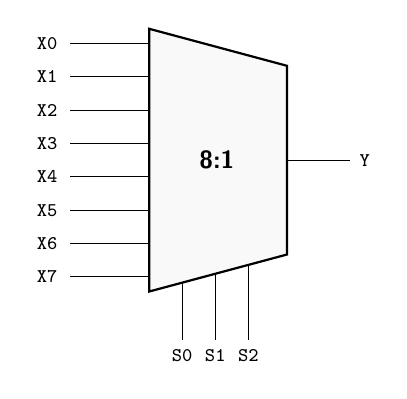
\begin{tikzpicture}[x=1cm,y=.47cm,font=\scriptsize\ttfamily]
\draw[line width=.8pt,fill=gray!5](1,0)--(2.75,1.0)--(2.75,6.1)--(1,7.1)--cycle;
\foreach \i in {0,...,7}{\pgfmathsetmacro{\yy}{6.7-.9*\i}\draw(0,\yy)--(1,\yy);\node[anchor=east]at(-.04,\yy){X\i};}
\draw(2.75,3.55)--(3.55,3.55)node[right]{Y};
\node[align=center,font=\sffamily\bfseries\small]at(1.86,3.55){8:1};
\foreach \i in {0,1,2}{\pgfmathsetmacro{\xx}{1.42+.42*\i}\draw(\xx,-1.3)--(\xx,.23+.24*\i);\node[below]at(\xx,-1.3){S\i};}
\end{tikzpicture}
\Caption{LOGIC SYMBOL. Functional diagram; signal names identify the connections.}
\end{minipage}
\section*{Logical connections and selection}
\begin{minipage}[t]{.56\linewidth}\vspace{0pt}
\par\noindent\begin{tabularx}{\linewidth}{@{}l l Y@{}}
\toprule\TableHead Signal & Direction & Function\\\midrule
$X_0$--$X_7$ & In & Eight independent digital levels.\\
$S_0$--$S_2$ & In & Binary channel selection; $S_0$ has weight one.\\
$Y$ & Out & Delayed copy of the selected level.\\\bottomrule
\end{tabularx}\par
\vspace{7pt}
\textbf{No hidden control pin.} This logical contract defines no enable, latch, clock, or serial protocol. This document covers the digital selection interface.
\end{minipage}\hfill
\begin{minipage}[t]{.38\linewidth}\vspace{0pt}
\centering\begin{tabular}{cccc}
\toprule\TableHead $S_2$ & $S_1$ & $S_0$ & Settled $Y$\\\midrule
\MuxTruthRows
\bottomrule
\end{tabular}
\Caption{Truth table applies after settling with valid, driven inputs.}
\end{minipage}
\vfill
{\scriptsize\color{Muted}DOCUMENT CONTROL / P3. Interface revision 02 retained; selection and settling behavior unchanged.}
\clearpage
\Continuation{Switching characteristics}{A stable interval is required after the latest relevant transition.}
\MetaStrip{\PartNumber\hfill \DocumentNumber\hfill INTERFACE REVISION 02}
\par\noindent\begin{tabularx}{\linewidth}{@{}l Y c l@{}}
\toprule\TableHead Symbol & Characteristic & Value & Unit\\\midrule
$t_s$ & Settling after a select change & \SettlingUs & $\mu$s\\
$t_s$ & Settling after a selected-input change & \SettlingUs & $\mu$s\\
--- & Output during settling & \multicolumn{2}{l}{Previous resolved value}\\
--- & Further relevant transition & \multicolumn{2}{l}{Restart the interval}\\\bottomrule
\end{tabularx}
\Caption{Specified interface settling interval. An unselected input transition alone does not change the selected channel.}
\section*{A. A selection changes; the selected input stays low}
Initially $Y$ is high. At $t=0$, a channel with a stable low input is selected. The prior output persists until $t=2~\mu$s.
\begin{center}
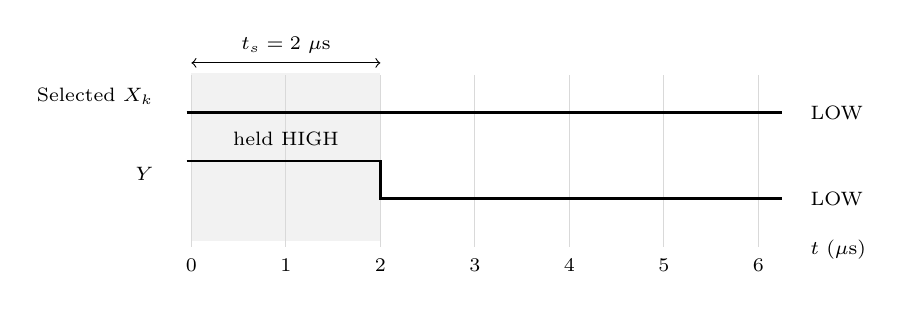
\begin{tikzpicture}[x=1.2cm,y=.68cm,font=\scriptsize]
\fill[gray!10](0,-.25)rectangle(2,2.9);
\foreach \x in {0,1,...,6}{\draw[gray!30](\x,-.35)--(\x,2.85);\node[below]at(\x,-.4){\x};}
\node[anchor=east]at(-.3,2.45){Selected $X_k$};\node[anchor=east]at(-.3,1){$Y$};
\draw[line width=1pt](-.05,2.15)--(6.25,2.15);
\draw[line width=1pt](-.05,1.25)--(2,1.25)--(2,.55)--(6.25,.55);
\draw[<->](0,3.08)--(2,3.08)node[midway,above]{$t_s=2~\mu$s};
\node[anchor=west]at(6.45,2.15){LOW};\node[anchor=west]at(6.45,.55){LOW};
\node[anchor=west]at(6.45,-.4){$t$ ($\mu$s)};
\node[font=\scriptsize]at(1,1.66){held HIGH};
\end{tikzpicture}
\end{center}
\section*{B. A later transition restarts the settling interval}
Initially $Y$ is high. The selected input goes low at $t=0$, high at $t=1$, then low at $t=3$. The output first becomes low at $t=5~\mu$s$\,$: two microseconds after the latest transition.
\begin{center}
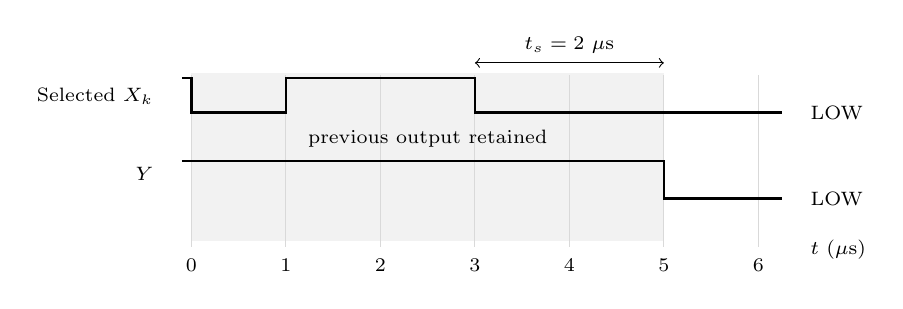
\begin{tikzpicture}[x=1.2cm,y=.68cm,font=\scriptsize]
\fill[gray!10](0,-.25)rectangle(5,2.9);
\foreach \x in {0,1,...,6}{\draw[gray!30](\x,-.35)--(\x,2.85);\node[below]at(\x,-.4){\x};}
\node[anchor=east]at(-.3,2.45){Selected $X_k$};\node[anchor=east]at(-.3,1){$Y$};
\draw[line width=1pt](-.10,2.8)--(0,2.8)--(0,2.15)--(1,2.15)--(1,2.8)--(3,2.8)--(3,2.15)--(6.25,2.15);
\draw[line width=1pt](-.1,1.25)--(5,1.25)--(5,.55)--(6.25,.55);
\draw[<->](3,3.08)--(5,3.08)node[midway,above]{$t_s=2~\mu$s};
\node[anchor=west]at(6.45,2.15){LOW};\node[anchor=west]at(6.45,.55){LOW};
\node[anchor=west]at(6.45,-.4){$t$ ($\mu$s)};
\node[font=\scriptsize]at(2.5,1.66){previous output retained};
\end{tikzpicture}
\end{center}
\begin{Notice}{SETTLING IS NOT SOFTWARE DEBOUNCE}
A short pulse may not reach the output, but the specified microsecond settling behavior is not a debounce guarantee. Contact bounce and stable button recognition remain separate application concerns.
\end{Notice}
\vfill
{\scriptsize\color{Muted}Timing diagrams show deliberately chosen starting conditions. They do not add a universal power-on output guarantee.}
\clearpage
\Continuation{Integration and verification}{Signal integrity at the interface, acquisition sequence and functional checks.}
\MetaStrip{\PartNumber\hfill \DocumentNumber\hfill DOCUMENT ISSUE\ \PresentationRevision}
\section*{Connection discipline}
Drive the three address inputs and read $Y$ as an input. Establish valid levels on every source that may be selected. Update the address, allow settling, then sample the result. Changing address bits individually can produce intermediate selections; begin the settling allowance after the final relevant transition.

A contact-to-ground application may use pull-ups so that closure reads low. That polarity comes from the surrounding wiring, not the multiplexer. Consult the equipment wiring drawing for controller pins and independent inhibit circuits.
\section*{Undefined input conditions}
\par\noindent\begin{tabularx}{\linewidth}{@{}l Y@{}}
\toprule\TableHead Condition & Interface consequence\\\midrule
LOW or HIGH & A defined digital value can be sampled.\\
High impedance & The net requires a bias or another valid driver to resolve a defined level.\\
Opposing driven levels & The resulting level is undefined; avoid output contention.\\
Floating or contended sample & No defined logic result is available until the input is correctly biased and driven.\\\bottomrule
\end{tabularx}
\Caption{The MX8-1 does not provide current limiting or a contention-protection function. A defined logic value requires a valid, resolved source.}
\section*{Functional verification schedule}
\par\noindent\begin{tabularx}{\linewidth}{@{}l Y Y@{}}
\toprule\TableHead ID & Stimulus & Required observation\\\midrule
M01 & Select each of eight channels with defined inputs. & The settled result matches the truth table.\\
M02 & Change selection to the opposite level. & Previous output before $t_s$; new value after settling.\\
M03 & Change the selected input within $t_s$. & Latest transition restarts the interval.\\
M04 & Toggle an unselected input only. & No selected-channel output change.\\
M05 & Route a bouncy contact. & No promise of debounced button events.\\
M06 & Check source bias and output direction. & Every sampled signal has a defined driver or bias; no opposing output drivers.\\\bottomrule
\end{tabularx}
\section*{Acquisition sequence}
Establish the final address on S2:S0. Allow at least $t_s$ after the last address transition or selected-input transition before accepting a new output level. If the source is a mechanical contact, qualify its stable state separately over the applicable contact-bounce envelope.

An eight-channel scan is time-distributed: channel zero and channel seven are not sampled at the same instant. A system that compares several channels must account for changes that occur between those acquisitions.
\vfill
{\scriptsize\color{Muted}TriAxis Logic / MUX-001 / Interface revision 02 / Document issue \PresentationRevision.}
\end{document}
